Galois Theory is a popular and one of the important theory in Abstract Algebra. It's foundation was first laid by the French Mathematician \textit{Évariste Galois} by determining the necessary and sufficient condition for solving the polynomial equation by radicals and thereby solving the problem that was open for 350 years old.\\ \\
The core-part of the Galois Theory is the \textit{Fundamental Theorem} of Galois Theory which links two main parts of Abstract Algebra; Field Theory and Group Theory. This is a profound result in Abstract Algebra. \\

\section{Approaches to the Theory}
\begin{enumerate}
\item Galois approached this problem by using the properties of permutation groups to the roots of a
polynomial equation solvable by radicals. And this linked Field theory to Group theory.
\item The modern approach is to use the field extension of the underlying field of the polynomial and
examine the groups of automorphism of the extension field that fixes the underlying field.
\end{enumerate}

\clearpage

\section{Life History of Galois}

He was Born in an educated family in Paris in the era of Napoleon. Napoleon was at the height of his power in 1811 but by 1824 his French empire was falling apart and he was put into prison by the British.\\ \\
Galois was by this time at school and enrolled in mathematics class in 1827(16 yrs) where he was described intelligent, singular and original. In 1829(18 yrs) he published his first paper on continued fractions and submitted his articles on the algebraic solution of equations where
\textit{Cauchy} was a referee of Galois’ paper. He again submitted a new article which was sent to \textit{Fourier}, to be considered for the Grand Prize in mathematics but Fourier died and Galois’ paper was never found.\\ \\

\begin{wrapfigure}{r}{0.27\textwidth}
  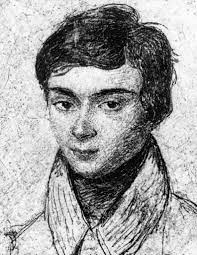
\includegraphics[scale=0.7]{galois.jpg}
  \caption{Galois}
\end{wrapfigure}

He was frustrated, and then became involved in the political revolution going on then in France against Napoleon. He got arrested was put into prison where he fell in love with \textit{Stephanie}. He then fought a duel with \textit{Prscheux} who was a solder. The reason of the fight is not clear. It is guessed that both of them loved Stephanie. He got shot in the duel and died the other day.\\ \\
There is this legend that he spent his last night writing all he knew about group theory. Galois’ papers were sent to Gauss,Jacobi and others. Later the paper reached to Liouville who published them in 1846.